\documentclass[../sparc.tex]{subfiles}
\graphicspath{{\subfix{../images/}}}
\begin{document}

%%%%%%%%%%%%%%%%%%%%%%%%%%%%%%%%%%%%%%%%%%%%%%%%%%%%%%%%%%%%%%%%%%%%%%%%%%%%%%%%
\section{Analog ports}
\label{section:analog-ports}

On Arduino boards we can find so called \emph{analog ports} that allow us to
read analog signals.  On the board, they labeled as \texttt{A0}, \texttt{A1}
etc.  While \emph{digital ports} are used for reading digital signals that can
be in two states (0V or 5V), \emph{analog ports} are used accordingly for
reading analog, continuous signals that can take any value in the 0..5V range.

As the first example we will try to send analog values to a computer from an
analog port that is not connected anywhere.

In the code we will be using \texttt{analogRead} (see the listing
\ref{listing:analog-ports-get-value}.)

\begin{listing}[ht]
  \begin{minted}{cpp}
    void setup() {
      Serial.begin(9600);
    }

    void loop() {
      // Getting the value from the analog port 0.
      int value = analogRead(A0);

      Serial.println(value);

      delay(100);
    }
  \end{minted}
  \label{listing:analog-ports-get-value}
  \caption{Getting the value from an analog port.}
\end{listing}

If we upload the code from the listing \ref{listing:analog-ports-get-value} to
an Arduino and check the serial monitor in Arduino IDE, we will see that the
signal takes values that are completely random on the first glance.
Nevertheless we can affect the signal -- if we move our hand closer to the
Arduino, we will likely see that the signal changes as we move our hand.  Does
it mean that we discovered some super ability and we have to sign in to the
super-heroes league?  Unfortunately, no -- but still we just discovered an
ability in Arduino to read electromagnetic noise that is usually hidden from us
in the everyday life.

There are several ways to ``see'' this nose in everyday life.  For example we
can adjust an analog radio to the frequency between radio stations to hear the
``hissing'' noise from the radio speaker.  An example of such noise is shown on
fig. \ref{fig:white-noize}.

\begin{figure}[ht]
  \centering
  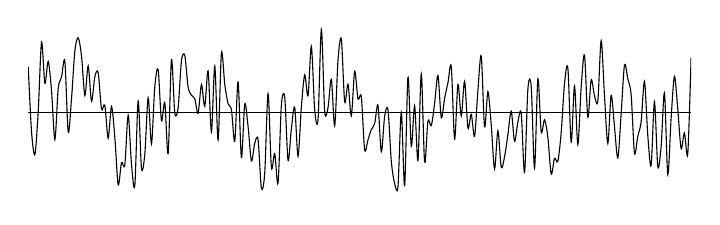
\begin{tikzpicture}[samples=200, domain=0:5*360]
    \begin{axis}[
        width=10cm, height=4cm,
        enlarge x limits=false,
        xtick=\empty,
        axis lines*=middle,
        hide y axis
      ]
      \addplot [no markers, smooth] {sin(x)+rand*2};
    \end{axis}
  \end{tikzpicture}
  \caption{White noise.}
  \label{fig:white-noize}
\end{figure}

As strange as it may sound, there are different ``colors'' of noise: ``white'',
``pink'', ``red'', ``violet'' and ``gray''.  Noises of different ``colors''
differ in the spectrum of the signal and the ``color'' characteristic is given
to it by analogy to the spectrum of visible light.  In our case we discuss only
the ``white'' noise that also gave the name to this chapter of the book.

``White'' noise is a signal, the components of which is spread evenly across the
used range of frequencies.  If we would play the ``white'' noise through a
speaker we would hear that all the audible sound frequencies are presented
evenly -- in other words we would hear only ``shhh'' sound from the speaker.

\note{ The image \ref{fig:white-noize} is generated at the time of the building
  the digital version of the book in PDF format and in different versions of the
  book the image will differ from the others.  That is because we used random
  number generator to generate this image and usually the source of randomness
  in a computer is the unpredictability of the real world; in particular, as we
  discussed above, the ``white'' noise is source of such unpredictability. }

As in case with an Arduino such noises are captured by the circuit itself and
converted to the numbers of specified range.

Such an electromagnetic background is constantly existing around us; and it has
many sources.  Firstly, such noise is created by the human civilization
altogether -- TV and radio-transmitter towers; base stations that providing the
cell network services; the mobile phones themselves that transfer data through
wireless networks and so on.  Secondly, there are completely natural sources of
radio waves -- for example, some kinds of stars produce very strong radio
signals.

For convenient observation of the signal we can use the ``Serial plotter'' from
the ``Tools'' menu -- this way we can see the graph similar to
\ref{fig:white-noize}.

\experiment{0}{ Try to bring your mobile phone closer to the Arduino.  Does the
  signal change? }

\experiment{1}{ Try to connect \texttt{A0} to the ground (``GND'' port), then
  disconnect it from the ground and connect \texttt{A0} to ``5V'' port on the
  Arduino.  What happens to the signal? }

Do we have any good use for such noise?  It happens to be yes, we do.  Thanks to
the unpredictability of the noise it can be used as the source of random numbers
-- which is useful, for example, in the game development which we discuss in the
following chapters of the book.

\subsection{Exercises}

\begin{enumerate}
\item Modify the source code from the example \ref{listing:serial-port-sine-wave-example}
  to control the sine wave parameters using a potentiometer.
\end{enumerate}

\end{document}
